
\iffalse
\begin{forest}
  for tree={
    font=\ttfamily,
    grow'=0,
    child anchor=west,
    parent anchor=south,
    anchor=west,
    calign=first,
    inner ysep=0pt,
    edge path={
      \noexpand\path [draw, \forestoption{edge}]
      (!u.south west) +(20pt,0) |- node[fill,inner sep=5pt] {} (.child anchor)\forestoption{edge label};
    },
    before typesetting nodes={
      if n=1
        {insert before={[,phantom]}}
        {}
    },
    fit=band,
    before computing xy={l=40pt}, % Horizontal line length
  }
[
  [\myfolder{NXinstrument}
    [\myfolder{NXsource}]
    [\myfolder{NXdetector}
        [\myfile{counts[100]}]
        [\myfile{gas\_pressure[100]}]
        [\myfile{two\_theta[100]}]
        [\myfolder{NXoff\_geometry}
            [\myfile{vertices[100]}]
            [\myfile{faces[100]}]
        ]
    ]
    [\myfolder{NXmonochromator}]
  ]
  [\myfolder{NXdata}
    [\myfile{counts[100]}]
    [\myfile{two\_theta[100]}]
  ]
  [\myfolder{NXsample}]
]
\end{forest}
\fi

\begin{figure}
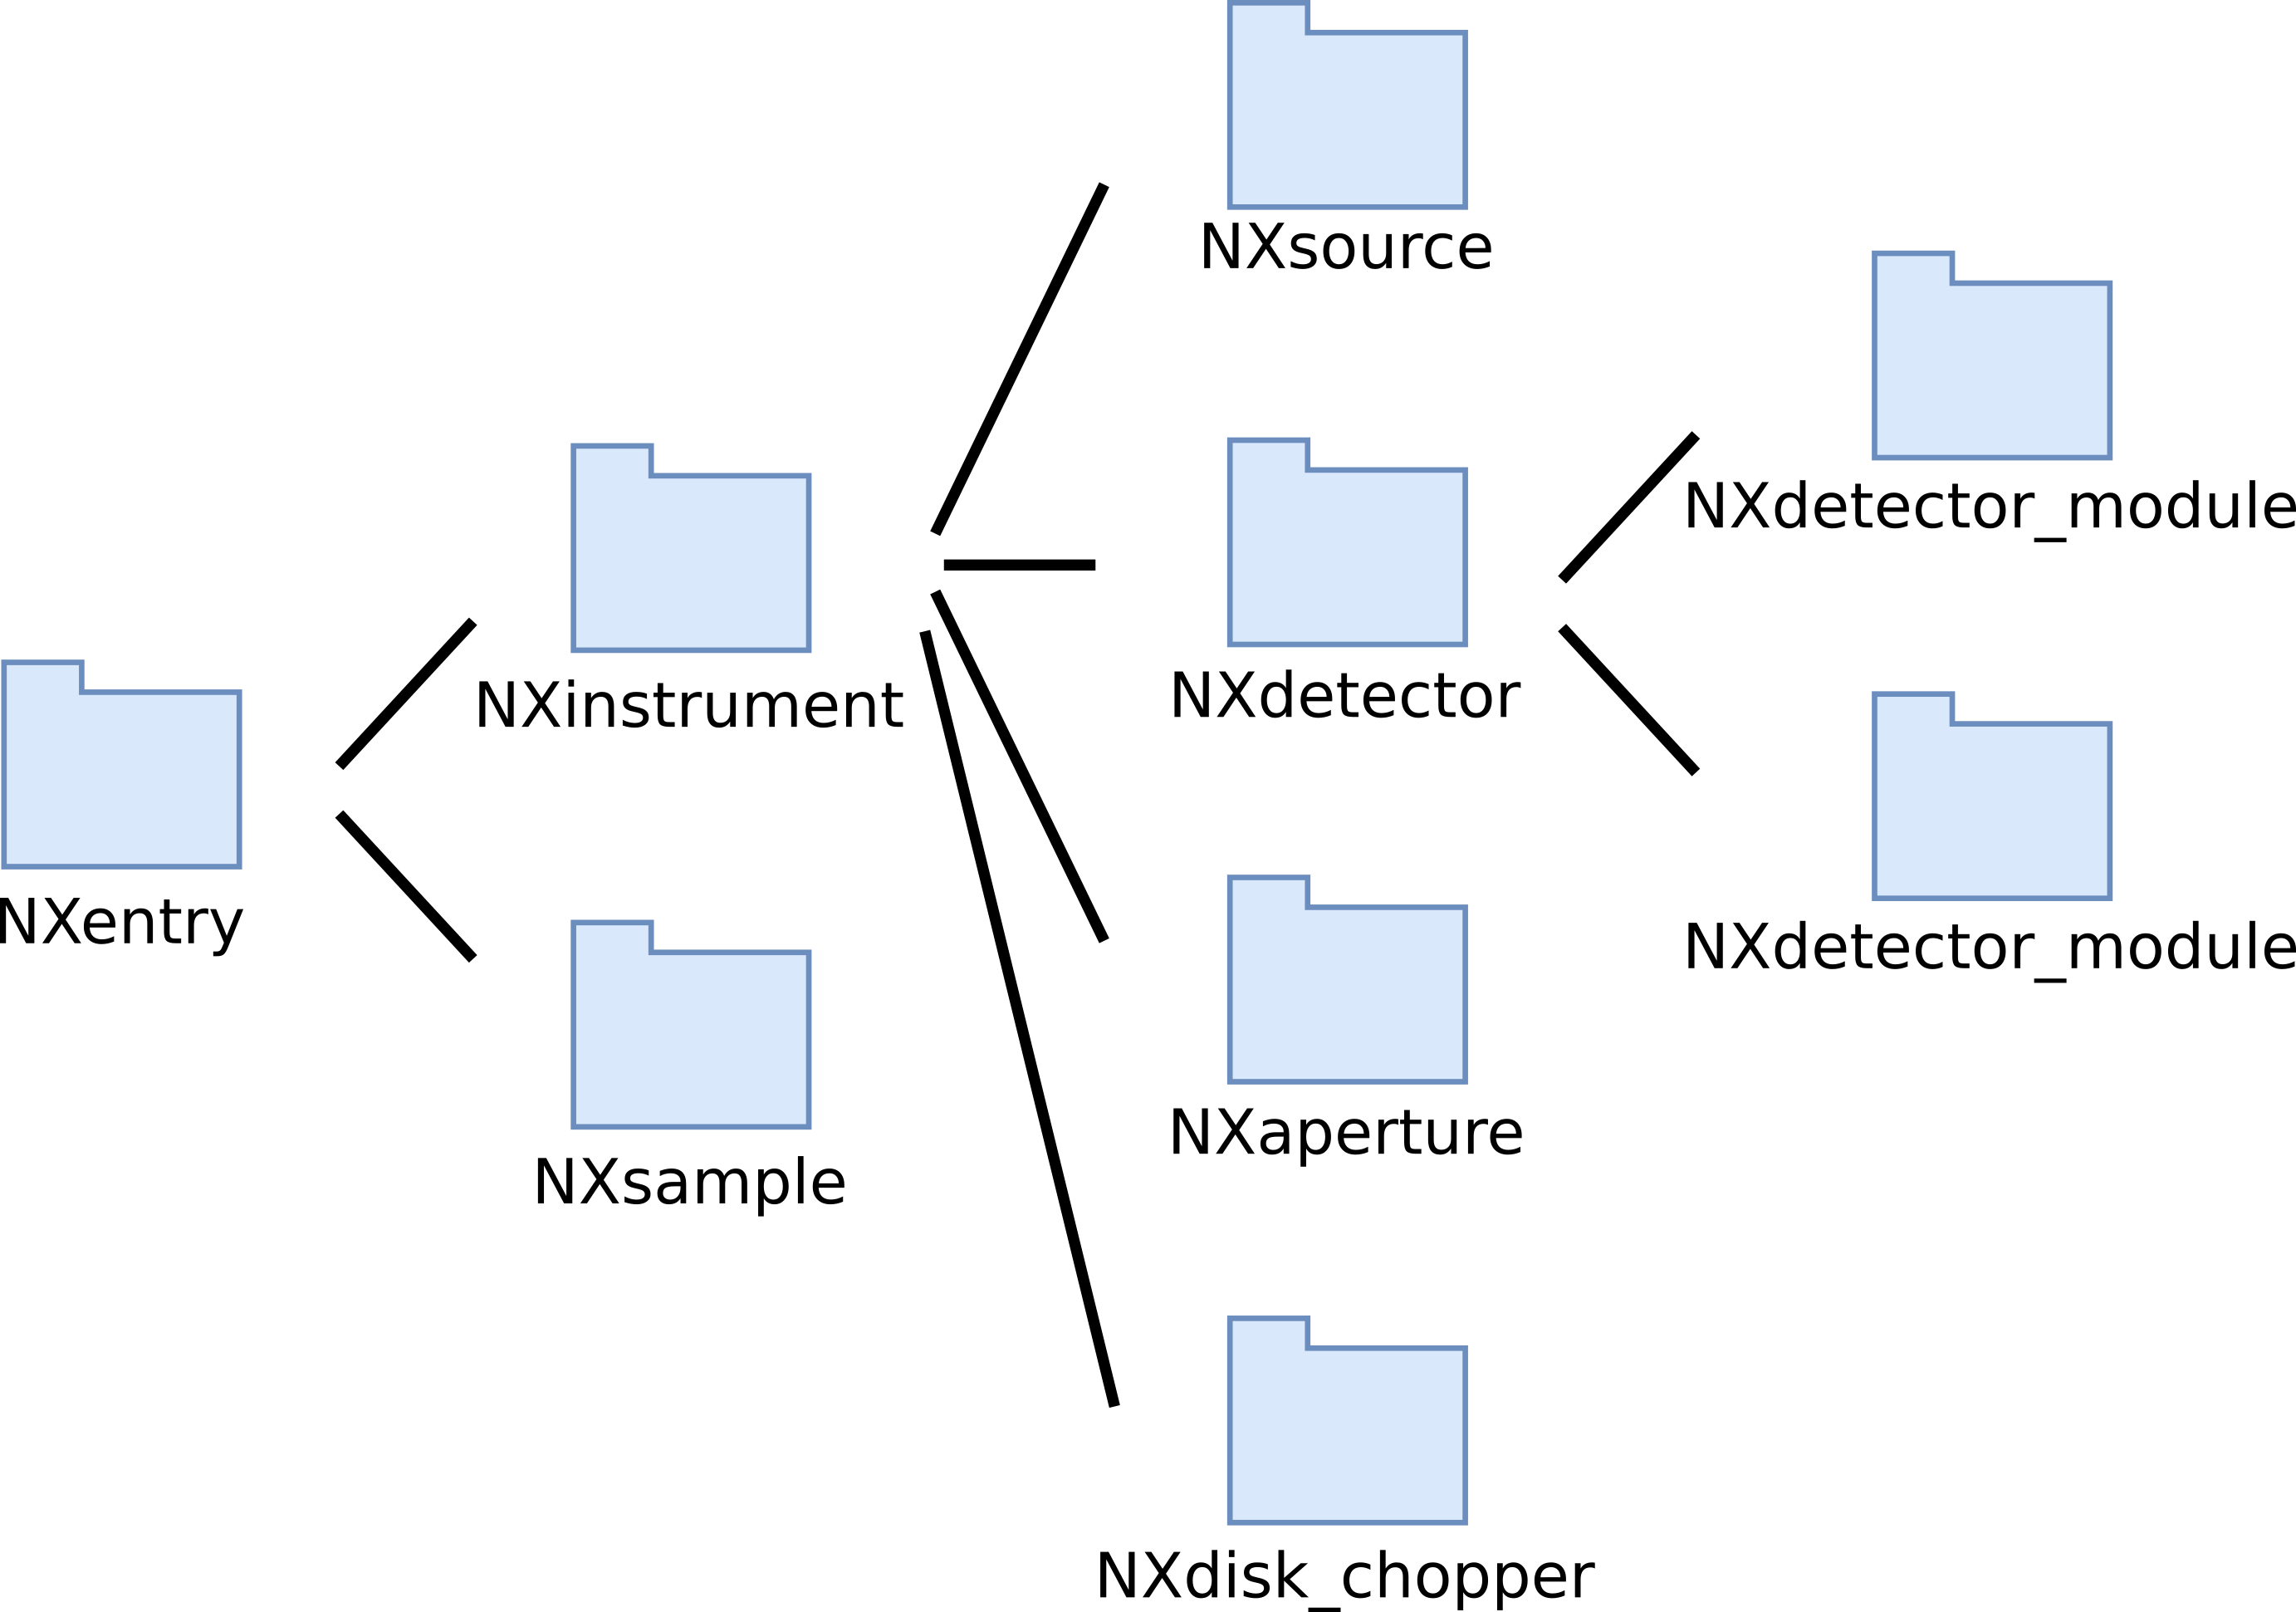
\includegraphics[width=0.7\linewidth]{instrument_arch.png}
\caption{A typical NeXus file layout}
\end{figure}

% What's a shape definition?

The NeXus file format was developed with the following aims:
\begin{itemize}
\item to create a file format which is common to different neutron facilities,
\item to store all experiment data in a single file,
\item to create a file format which can be read into various different software 
\end{itemize}

\iffalse
A recent addition to the NeXus standard means components that are used in experiments can specify shape definition to describe their placement, size and geometry. Transformations (NXtransformations) can be applied to these components when their position changes during or before the experiment.
\fi
